\section{Workloads}
\label{sec:approach}

This section presents the data placement problem.
First, it characterizes the workloads used in the work.
Next, it expounds on the three dimensions of the problem:
(1) granularity, (2) replication, and (3) placement.
Last, it explains and analyzes three data placement methods,
comparing
performance in terms of load imbalance, storage footprint, and robustness.

\subsection{Workload Characteristics}
\label{sec:workloads}

A workload can be described with several critical characteristics,
such as arrival rate and autocorrelation.
Because this work considers data replication and placement, 
the workload characteristic that matters most is access frequency of the
individual elements of the
dataset, such as, the pages of a web server or the keys in an index.
Other characteristics are not factored into
this work because they do not have a direct impact on data replication
or placement.

A uniform workload is atypical and likely artificial,
which is unsurprising because
non-uniform workloads are common in many natural settings
~\cite{Pavlo2012}.
For example, the normal (Gaussian) distribution can be observed
in class score distribution,
while the log-normal distribution is useful to describe
the response file size in web servers~\cite{Barford1998}.
In addition, the power law probability distribution is widely applicable to
web hits, word frequency, personal income, \emph{etc}.\ and tends to
be highly skewed towards a small subset of the full
dataset~\cite{Newman2005}.
That is, a small number of partitions accounts the vast majority of key access
and most of the partitions are touched infrequently. 
Several studies show that frequency of access to different pages or
keys often follows a Zipf or power law distribution.
This has been shown in web servers~\cite{dilley1998web,panteleenko2003web},
video streaming~\cite{sripanidkulchai2004analysis}, 
and Wikipedia traffic~\cite{urdaneta2009wikipedia} to name a few.

In this work, we consider the
\emph{normal} and the \emph{power law} distribution for their
wide appearance in many workloads.
We also consider the \emph{uniform} distribution for a n\"aive baseline,
\emph{beta}, which is less skewed than
\emph{normal} and \emph{power law}, and
\emph{gamma}, which generates the highest skewed workload and
has been used in modeling workloads in storage systems~\cite{Wilkes2001}.


\mytable{\ref{tab:load-imbalance}} shows
the five workload distributions used in the work.
This table presents the distribution of the
requests on each of four partitions ($M=4$, $k=1$).
There are 30,000 unique requests among the 1024 keys,
and the average is 7,500 requests per partition.
The requests-per-node values are ordered in decreasing magnitude.
As expected there are approximately the same number of requests for
each partition in the uniform distribution.
The \emph{max:mean} column shows the ratio of the maximum number of requests
to the average.
Because the total running time is largely dependent on the slowest or
most heavily loaded node, the max-mean ratio foretells the performance
penalty for each workload on a uniform distribution.
The ratio for uniform is 1.01, meaning the maximum is 1\% greater
than the average.
But the highly-skewed gamma distribution has one partition that receives
no requests and one has more than three times the average.
It is clear from \mytable{\ref{tab:load-imbalance}} that in
non-uniform workloads
the maximally loaded partition demands
more resources than the other partitions.
The final column presents access imbalance using the 
\emph{skew} metric~\cite{Pavlo2012}. 

This work evaluates the problem using synthetic workloads.
An alternative is to evaluate using real-world traces.
But such traces are in short supply.
Moreover, a trace represents a very specific situation that may not be
representative of a general class.
Additionally, a trace has many characteristics that are hard to
control.
Using synthetic workloads enables us to evaluate more distributions and
confine the observed effects to the change in distribution.


\begin{figure}[!htbp]
\begin{subfigure}[b]{0.45\textwidth}
    \includegraphics[width=\linewidth]{figures/E45_simulation_imbalance_coarse_std_uniform.eps}
    \caption{uniform}
\end{subfigure}
\begin{subfigure}[b]{0.45\textwidth}
    \includegraphics[width=\linewidth]{figures/E45_simulation_imbalance_coarse_std_beta.eps}
    \caption{beta}
\end{subfigure}
\begin{subfigure}[b]{0.45\textwidth}
    \includegraphics[width=\linewidth]{figures/E45_simulation_imbalance_coarse_std_powerlaw.eps}
    \caption{power law}
\end{subfigure}
\begin{subfigure}[b]{0.45\textwidth}
    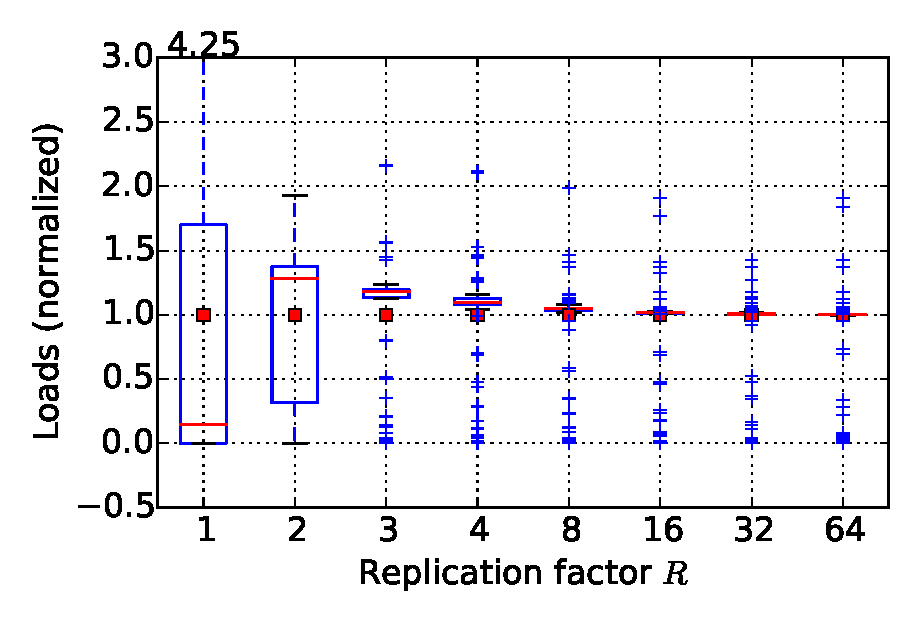
\includegraphics[width=\linewidth]{figures/E45_simulation_imbalance_coarse_std_normal.eps}
    \caption{normal}
\end{subfigure}
\begin{subfigure}[b]{0.45\textwidth}
    \includegraphics[width=\linewidth]{figures/E45_simulation_imbalance_coarse_std_gamma.eps}
    \caption{gamma}
\end{subfigure}
\centering
\caption{The load distribution among nodes under the coarse-grain data placement ($M=64, k=1$).}
\label{fig:simulation_imbalance_coarse}
\end{figure}


\begin{figure}[!htbp]
\begin{subfigure}[b]{0.45\textwidth}
    \includegraphics[width=\linewidth]{figures/E45_simulation_imbalance_fine_std_uniform.eps}
    \caption{uniform}
\end{subfigure}
\begin{subfigure}[b]{0.45\textwidth}
    \includegraphics[width=\linewidth]{figures/E45_simulation_imbalance_fine_std_beta.eps}
    \caption{beta}
\end{subfigure}
\begin{subfigure}[b]{0.45\textwidth}
    \includegraphics[width=\linewidth]{figures/E45_simulation_imbalance_fine_std_powerlaw.eps}
    \caption{power law}
\end{subfigure}
\begin{subfigure}[b]{0.45\textwidth}
    \includegraphics[width=\linewidth]{figures/E45_simulation_imbalance_fine_std_normal.eps}
    \caption{normal}
\end{subfigure}
\begin{subfigure}[b]{0.45\textwidth}
    \includegraphics[width=\linewidth]{figures/E45_simulation_imbalance_fine_std_gamma.eps}
    \caption{gamma}
\end{subfigure}
\centering
\caption{The load distribution among nodes under the fine-grain data placement with various $k$ ($M=64, R=2$).}
\label{fig:simulation_imbalance_fine}
\end{figure}


\begin{table}[!htbp]
  \centering
  \caption{Load-imbalance of workloads.}
  \resizebox{\columnwidth}{!}{%
  \begin{tabular}[h]{lrrrrcc}
    \toprule
Distribution & 	\multicolumn{4}{l}{Requests for individual partitions}
    & max:mean & skew\\
\midrule
Uniform & \textbf{7,565} & 7,548 & 7,449 & 7,438 & 1.01 & 0.15\\
Beta & \textbf{10,313} & 10,288 & 4,715 & 4,684 & 1.38 & 0.39\\
Power law & \textbf{17,344} & 8,795 & 3,361 & 500 & 2.31 & 0.60 \\
Normal & \textbf{14,882} & 14,827 & 149 & 142 & 1.98 & 0.74\\
Gamma & \textbf{23,542} & 6,329 & 129 & 0 & 3.14 & 0.77\\
\bottomrule
  \end{tabular}
  }
  \label{tab:load-imbalance}
\end{table}


%%%%%%%%%%%%%%%%%%%%%%%%%%%%%%%%%%%%%%%%
% Approaches
%%%%%%%%%%%%%%%%%%%%%%%%%%%%%%%%%%%%%%%%

\subsection{Data Placement Steps}
\label{sec:dp_methods}

A data placement method requires determining
partition granularity, replication factors, and placement schemes.
Partition granularity represents the smallest unit
for replicating data and calculating loads.
The coarsest granularity is one partition per node ($k=1$), and
the finest is one partition per key.
A small $k$ decreases the likelihood of balancing a non-uniform workload.
However, a large $k$ increases management overhead.

Once the partition granularity $k$ is determined,
the next step
in deriving a solution is determining the number of
replicas for each partition based on the expected workload.
For example, suppose there are four partitions ($P=4$) with a
replication factor of four ($R=4$), then
there are sixteen slots for these partitions ($S=16$) in a
coarse-grain solution.
Given a uniform expected workload the replication factor vector would be 
[4, 4, 4, 4], that is there are four copies of each of the four
partitions. 
For a workload with a normal distribution the replication factor
vector might be [2, 6, 6, 2] and for 
power law it might be [1, 2, 4, 9].
In general, there is no perfect match between the vector and the
anticipated workload.

Assuming that the predicted load on each partition is $\lambda_i$ and the total
load is $\Lambda = \sum_{i=1,P}\lambda_i$.
The replication problem is to determine the \emph{replication vector},
$\vec{R}, R_i \in \mathcal{I}$, such that
$R_i \ge 1~\forall i$  and
$S = \sum_{i=1,P}R_i$.
In words, the replication vector contains the number of replicas (an
integer value) of each partition, such that the total number of
replicas equals the number of slots available.
The replication error is
$E = \sum_{i=1,P} | R_i/S - \lambda_i/\Lambda |$, which is the
accumulation of difference between 
the actual relative
replication of each partition ($R_i/S$) and
the anticipated relative
workload per partition ($\lambda_i/\Lambda$).

%\input{tables/delta_powerlaw}

The last step is assigning the replicas to the slots on the nodes.
For coarse-grain, the number of replicas equals the number of
slots and there is only one possible placement.
But for fine-grain, $k>1$, there are many possible placements.
One placement strategy is to minimize the number of unique
partitions on each node in order to reduce dataset footprint on the
nodes.
We call this strategy \emph{compact}.
If there are multiple choices,
it picks the node with the least load.
The opposite strategy to \emph{compact} is \emph{full},
which maximizes the number of different partitions on each node and
also picks the node with the least load.
The third strategy is placing partitions in order to balance loads as much as possible.
We call this strategy \emph{balanced}. 
We show that although \emph{full} and \emph{balanced} have
different goals, the resultant placements and effects are similar.
Furthermore, \emph{compact} and \emph{full}
balance loads among the
nodes with their best efforts within their given constraints.
Consequently, all three strategies achieve good load balancing, of
course \emph{balanced} is a slightly better at it.
To reiterate:
The goal of \emph{compact} is reducing the number of unique partitions
on each node, which reduces the 
footprint of the data set.
On the other hand, the goal of \emph{full} is to distribute
replicas for the same partition to as many nodes as possible---balancing
the load---with the intent of increasing the availability of hot partitions. 



Our data placement procedure is described in Algorithm \ref{alg:dp}.
This is a framework and therefore, different placement strategies can be used.
The complexity for generating the replication vector is proportional
to the number of partitions, $\mathcal{O}(Mk)$.
Different placement strategies implement distinct
\emph{pick\_node} functions,
which is $\mathcal{O}(N)$.
This function is executed for each slot ($Nk$).
Therefore, the total complexity is of the placement algorithm
is $\mathcal{O}(kN^2)$.
Although it is quadratic, it is in the number of nodes that, even in a
very large cluster, is tractable.
A straightforward Python implementation executes in under few seconds
when $N=256$ and $k=16$.
Furthermore, this solution is a heuristic, it does not find the
optimal solution.
However, the solution is nearly optimal and because it is based on a
prediction of anticipated load optimal is unnecessary.


\begin{algorithm}[!htbp]
 \SetAlgoLined
 \DontPrintSemicolon
 \DontPrintSemicolon
 \KwIn{an historical workload}
 \KwOut{partition placement on each node}
 $M$ := the minimum number of nodes that hold all data\;
 $k$ := the selected partition granularity\;
 $R$ := the replication factor\;
 $loads$ := the predicted loads $\lambda_i$ of partitions\;
 $replicas$ := the replication vector (see Section~\ref{sec:model})

 \For{$p_i$ in $replicas$}{
   \For{$j$=1; $j<=p_i$; $j=j+1$}{
   	 /* strategy is \emph{compact}, \emph{balanced} or \emph{full} */\;
     n := pick\_node(strategy)\;
     assign $p_i$ to $n$
   }
 }
 \caption{Data Placement Procedure}
 \label{alg:dp}
\end{algorithm}




\subsection{Tradeoffs in Placement Strategy}
\label{sec:dp_tradeoff}

Our data placement framework is shown in Algorithm~\ref{alg:dp}.
This framework yields several variants of data placement
when choosing different placement strategies.
This section compares their effects on load balancing and storage footprint.

\subsubsection{Load Balancing}
The primary goal of data placement is distributing workloads evenly among nodes.
A highly skewed system is more likely to encounter performance bottlenecks.
Therefore, a well-balanced system achieves a higher system throughput.
To explore the benefit of fine-grain replication and placement, we
evaluate the effectiveness of 
our data placement schemes in balancing the anticipated workload.
We generated 100 instances of workloads, of 300,000 queries, for each of
the five distributions.
The workload instances vary because the access counts are generated
probabilistically.
Each generated workload is considered a prediction of the upcoming
workload.

First, we evaluate how the replication factor $R$ affects load balancing.
This simulation is conducted with $M=64$ and $k=1$.
We use the box plot, as shown in \myfigure{\ref{fig:simulation_imbalance_coarse}},
to analyze the loads distributed among nodes.
The bottom and top of the rectangle represent the first and third quartile of loads.
The red line is the median, and the red dot is the mean.
To facilitate comparison, the loads are normalized so that the means equal one.
Above the box is the whisker that is calculated by
adding $1.5$ times the interquartile range (IRQ) to the third quartile.
Similarly, the whisker below the box is the first quartile
minus $1.5$ times the IRQ.
The plus signs represent the data points that have the loads
beyond the two whiskers.
These is the standard representation for a box plot.
In a well balanced system, the median and mean values
will be close and the box will be small.

This figure clearly shows that increasing the replication factor
reduces load imbalance to a degree.
However, this alone is insufficient to eliminate
under-utilized loads totally because
increasing the number of replicas only reduces the loads.
The only way to reduce under utilization is
to overlap under and over utilized partitions,
which is not possible in the coarse grain method. 
Therefore, the replication factor alone is not sufficient
for balancing loads because it does not reduce under-utilization.
Take the \emph{gamma} distribution for example,
when $R=1$, most of the nodes are under utilized (low median) and
few nodes have extremely excess loads (large size box).
Doubling the replication factor creates more overloaded nodes
because $R=2$ is not enough to distribute loads.
As $R$ increases, the median value moves closer to the mean and
the variance (the size of box) also decreases,
which suggests over-utilization is mostly addressed.
However, increasing $R$ is still insufficient because
there are still many outliers (beyond the two whiskers).


Next, we examine how much the partition granularity can reduce load imbalance.
We run a set of simulations with $M=64$, $R=2$, and various $k$ values,
and choose \emph{balanced} as the placement scheme.
\myfigure{\ref{fig:simulation_imbalance_fine}} clearly shows that
fine partition granularity greatly reduces load imbalance.
Even in the most skewed workload (gamma), $k=16$ is able to almost perfectly balance loads.
For most workloads, $k=4$ is sufficient to reduce the load imbalance
below $10\%$.
When workloads are highly skewed (the \emph{normal} and \emph{gamma} case),
their load imbalance (the size of box in the figure) drops greatly from $k=1$ to $k=2$
because finer partitioning provides higher flexibility to mix
over- and under-utilized partitions on the same node.
Increasing partition granularity eventually leads to (for all
practical purposes)
perfectly balanced loads.


\begin{figure}[!htbp]
    \centering
    \includegraphics[width=0.8\textwidth]{figures/E42_simulation_colors_resized_powerlaw.eps}
    \caption{The number of unique partitions per node (storage footprint) under different placement schemes.}
    \label{fig:simulation_colors}
\end{figure}

\subsubsection{Storage Footprint}
There are $S=Nk$ choices for placing a partition replica.
When placing multiple replicas of the same partition on the same node,
it reduces the number of unique partitions per node.
When the number of unique partitions per node is lower,
it generally requires lower storage footprint.
A lower storage footprint reduces memory pressure, and may lead to higher cache efficiency.
We run a set of simulations with $M=64$, $R=2$ and various $k$.
This work only presents the results of the \emph{power law} workloads.
Other workload cases show very similar effects.

\myfigure{\ref{fig:simulation_colors}} shows the average number of
unique partitions on each node.
By definition all partitions in 
\emph{full} are unique and it is always 1 (normalized).
\emph{Balanced} is very nearly 1 in all cases.
On the other hand, as $k$ increases, 
\emph{compact} tends to $0.5$, which is $1/R$.
We further investigate how the replication factor affects storage footprint.
\myfigure{\ref{fig:simulation_colors_replication}} shows that the
number of unique partitions tends to $1/R$ as $k$ increases,
which is the desired outcome of the \emph{compact} scheme.


\begin{figure}[!htbp]
    \centering
    \includegraphics[width=0.8\textwidth]{figures/E42_simulation_colors_replication_resized_powerlaw.eps}
    \caption{The number of unique partitions per node under the \emph{compact} method with various $k$.  The number converges at $k=32$, which is equal to $1/R$.}
    \label{fig:simulation_colors_replication}
\end{figure}
